\documentclass[a4paper,12pt]{article}

\usepackage[english]{babel}
\usepackage[utf8]{inputenc}
\usepackage{amsmath,amsthm,amssymb,amsfonts,stmaryrd, wasysym}
\usepackage{color}
\usepackage{graphicx}
%%%%%%%%%%%%%%%%%%%%%%%% PRL-programm %%%%%%%%%%%%%%%%%%%%%%%%%
\usepackage{algorithm}
\usepackage{algpseudocode}
\usepackage{xcolor}
%%%%%%%%%%%%%%%%%%%%%%%% Kopf- & Fußzeile %%%%%%%%%%%%%%%%%%%%%%%%%
\usepackage[footsepline]{scrlayer-scrpage}
\pagestyle{scrheadings}
\clearscrheadfoot

\ihead{Machine Learning - Exercise 0}
\ifoot{\newline Christian Hatschka, Daniel Fangl, Esra Ceylan}
\ofoot{\newline \pagemark}

\begin{document}
\section{Group members}
	Daniel Fangl (01526097) has a bachelor in Software Engineering and is currently in the master course Software Engineering and Internet Computing. Christian Hatschka (01525634) and Esra Ceylan (01526801) have a bachelor in Mathematics and are currently in the master course Logic and Computation. 
	
\section{Choice of datasets}
	We looked for datasets with different characteristics. As a classification data\-set we chose one that is comparatively small in size but high in dimension. Moreover it has some missing values. In contrast, our regression dataset has a large size but small dimension and does not contain any missing values. Because of the diversity in size, dimension and expressibility we picked these two datasets.
	
	To put it in a nutshell, the choice of the datasets relates to the different sources of inexactness. While the small dataset could have errors in form of missing values or a small sample size, the large dataset is limited by its small number of dimensions.

\section{Classification dataset}
	For the classification dataset we chose 'Internet Advertisements Data Set' from UCI ML Repository (http://archive.ics.uci.edu/ml/datasets/Internet+ Advertisements). This dataset contains various information about the geometry of images, links as well as phrases occuring in advertisements on internet pages.
	
	The goal of the classification is to determine whether an element of a webpage is an advertisement.
	
	This dataset has a rather small sample size of $3279$ instances, whereas $2821$ are non-ads and $458$ are ads.	
	The small portion of advertisements seemed like a possible source of error in the dataset at first. After consideration, the reason for this is probably that the number of non-advertisement elements on an internet page is much bigger than the number of advertisement elements. Perhaps they were trying to reduce the number of false positives and were cautious with declaring ads. 
	
	Additionally, in our chosen dataset roughly $28$\% of the instances contain at least one missing attribute.
	
	Figure~\ref{fig:adsheight} shows a boxplot diagram of the distribution of heights of advertisements and non-advertisements. 
		\begin{figure}[h]
			\centering
			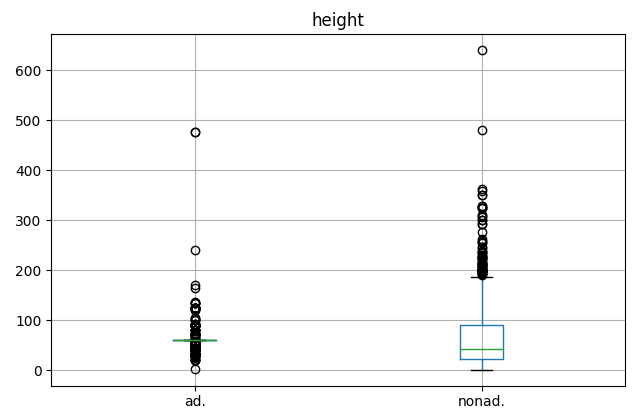
\includegraphics[width=0.7\linewidth]{images/ads_height}
			\caption{Boxplot of heights of (non-)advertisements}
			\label{fig:adsheight}
		\end{figure}
	
	Since this is a dataset from 1998, the data contained is relatively old and therefore might differ from todays advertisements. 

\section{Regression dataset}
	For the regression we selected the dataset 'Diamonds' from Open ML \newline (https://www.openml.org/d/42225). It contains general information about the diamond as well as e.g. it's price, weight or measurements. 
	
	The goal of the regression model is to predict the price of a diamond based on the given attributes. 
	
	The dataset has in total $53940$ samples, $10$ attributes and no missing values. The attributes can be divided into the following types: \\
	
	\begin{tabular}[h]{l|l}
		Ordinal & Cut (quality of the cut) \\
			& Color (worst to best) \\
			& Clarity (worst to best) \\
		\hline
		Interval & Table width (width from top relative to widest point)\\
			& Depth (a ratio of x, y, z) \\
		\hline
		Ratio & Carat (weight) \\
			& x, y, z (length, width, depth in mm) \\
			& Price (in US Dollars) 
	\end{tabular} \\
	
	The following figures show the distribution of the values of different attributes of the diamond dataset.
	%Below there are some graphs to show the distribution of values among the data types. 
	
	\begin{figure}[h]
		\centering
		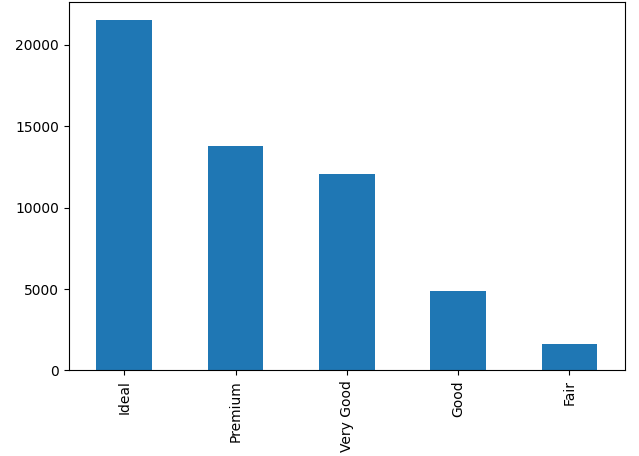
\includegraphics[width=0.7\linewidth]{images/diamond_cut}
		\caption{Quality of the cut}
		\label{fig:diamondcut}
	\end{figure}

	\begin{figure}[h]
		\centering
		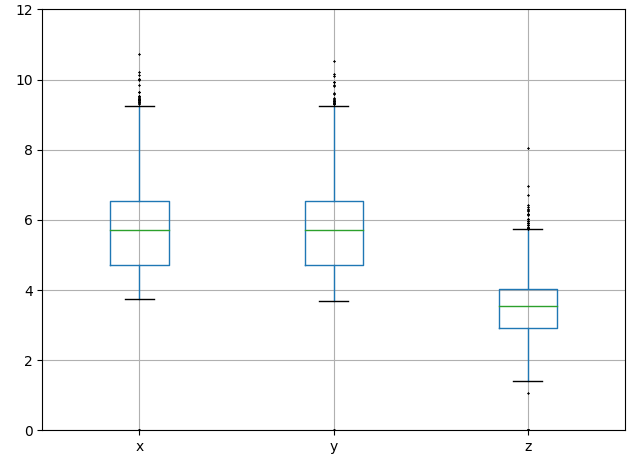
\includegraphics[width=0.65\linewidth]{images/diamond_axis}
		\caption{Boxplot of the length, width, depth of diamonds}
		\label{fig:diamondaxis}
	\end{figure}
\end{document}